\documentclass[conference]{IEEEtran}
\IEEEoverridecommandlockouts
% The preceding line is only needed to identify funding in the first footnote. If that is unneeded, please comment it out.
\usepackage{cite}
\usepackage{amsmath,amssymb,amsfonts}
\usepackage{multicol}
\usepackage{algorithmic}
\usepackage{graphicx}
\usepackage{textcomp}
\usepackage{listings}
\usepackage{xcolor}
\usepackage{listings}
\usepackage{url}

\def\BibTeX{{\rm B\kern-.05em{\sc i\kern-.025em b}\kern-.08em
    T\kern-.1667em\lower.7ex\hbox{E}\kern-.125emX}}
\begin{document}

\definecolor{mGreen}{rgb}{0,0.6,0}
\definecolor{mGray}{rgb}{0.5,0.5,0.5}
\definecolor{mPurple}{rgb}{0.58,0,0.82}
\definecolor{backgroundColour}{rgb}{0.95,0.95,0.92}

\lstdefinestyle{CStyle}{
	backgroundcolor=\color{backgroundColour},   
	commentstyle=\color{mGreen},
	keywordstyle=\color{blue},
	numberstyle=\tiny\color{mGray},
	stringstyle=\color{mPurple},
	basicstyle=\footnotesize,
	breakatwhitespace=false,         
	breaklines=true,                 
	captionpos=b,                    
	keepspaces=true,                 
	numbers=left,                    
	numbersep=5pt,                  
	showspaces=false,                
	showstringspaces=false,
	showtabs=false,                  
	tabsize=2,
	language=C,
	morekeywords={*,thread\_pool\_t, thread\_task\_t}
}

\title{Thread Pool in GeckoDB/BOLSTER - Implementing a Thread Pool for a High Performance Database System \\}

\author{
	\IEEEauthorblockN{Robert Jendersie, Johannes Wuensche, Johann Wagner, Marten Wallewein-Eising}
	\IEEEauthorblockA{\textit{Otto-von-Guericke University} \\
		Magdeburg, Germany \\
		\emph{firstname}.\emph{lastname}@st.ovgu.de} \and
}

\maketitle

\begin{abstract}
        Processing tasks in parallel is used in nearly all applications to keep
        up with the requirements of modern software systems. However, the
        current implementation of parallel processing in GeckoDB requires
        spawning many short-lived threads that execute a single task and then
        terminate. This creates a lot of overhead since the threads are not
        being reused. To counter this effect we implemented a thread pool to be
        used in GeckoDB to reduce the additional time required
        to create and close thousands of threads. In this paper, we show our
        implementation of a thread pool to process independent tasks in parallel,
        including the waiting for a set of processed tasks. We also compare the
        thread pool implementation against the current one. Additionally, we show that the task and thread pool configuration,
        depending on the use case, has a high impact on the thread
        pool performance. At the end of our evaluation, we show that the implementation 
        fulfils all given requirements and generally reduce
        overhead compared to creating and spawning threads individually.
\end{abstract}

\begin{IEEEkeywords}
Thread Pool, GeckoDB, BOLSTER
\end{IEEEkeywords}

\section{Introduction}
Since the amount of data that is stored and processed by modern database systems is growing fast, sequential data processing as only possibility is inconceivable. Applications have to process data in parallel to reach sufficient throughput to fulfil appropriate requirements.

Parallel data processing can be achieved by different approaches, like instruction and data parallelism or multi threading. In this paper, we focus on multi threading by implementing a thread pool for the graph database system GeckoDB. The thread pool will be integrated into BOLSTER, a high performance library for parallel execution of primitives like for or filter on large data sets. In the current implementation, BOLSTER creates a fix number of threads for each call of a primitive. This approach is called \emph{thread-per-request}. Since many primitives are executed at the same time, a couple of drawbacks arise from this implementation.
First of all, the creation of threads comes along with overhead like stack initialisation and memory allocation. Secondly, creating a huge number of threads simultaneously may lead to large context switch overhead of the scheduler. Additionally, debugging and profiling applications that create many threads during runtime is 	time-consuming.

To overcome these drawbacks, we integrate an optimised thread pool in BOLSTER. Along with the implementation, we measure the performance of the primitives to determine the thread pool overhead. Additionally, we measure metrics like \emph{waiting and busy time} of threads to evaluate correct thread pool sizes for the considered use cases. In this work we make the following contributions:
\begin{itemize}
	\item We describe our design and implementation of the thread pool
	\item We evaluate the possibility to wait for a group of task in the calling thread
	\item We compare our thread pool against the existing implementation in BOLSTER
	\item We measure and evaluate additional statistics for different thread pool configurations
\end{itemize}
We organized the rest of the paper as follows. In Section 2, we give preliminaries about the considered task configuration and about thread safe access of memory. In Section 3, we show our design and implementation of the thread pool and examine our experimental environment in Section 4. In Section 5, we describe the results of our performance evaluation. In Section 6, we name related work and state our conclusion and future work in Section 7.

\section{Preliminaries}
In this section, we define our configuration of tasks that are processed by the thread pool and state difficulties of synchronizing thread access to memory.

\begin{figure*}[htbp]
	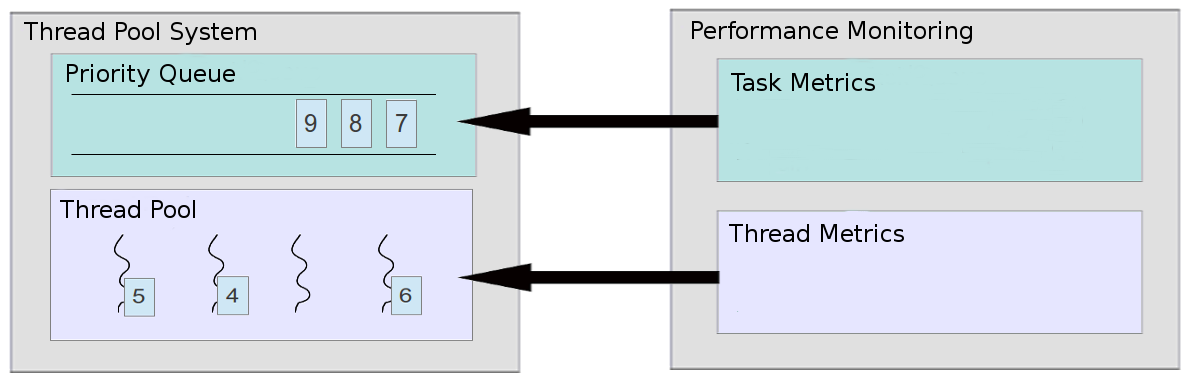
\includegraphics[width=1.0\textwidth]{img/pool_structure.png}
	\caption{Design of the thread pool system}
	\label{fig0}
\end{figure*}

\subsection{Task Configuration}
We define a Task as a structure referencing data that has to be processed and an operation that has to be executed on the data. In this work, we define tasks as \emph{independent}, which means tasks do not have dependencies on other tasks and can be processed independently. Furthermore, we expect the data passed to two tasks are stored in different memory locations. Consequently, while executing the task operation, threads do not access the same memory locations.

Each task can be enqueued with a priority. The priority zero is the highest and the task will be processed by the next free thread. The higher the priority of a task is, the further it is placed behind in the queue. Additionally, we only consider not preemtable tasks. Once a task is assigned to a thread, the thread will finish the operation of the task before getting a new one.

\subsection{Synchronizing Memory Access from Threads}
Parallelism with multi threading works great as long as each thread works on a separate memory location. During task scheduling, the scheduler has to know the state each thread has. This can be solved with signal handling or by writing the current thread state into main memory. In this work, we implement the second approach to avoid having another thread that only schedules tasks to other threads.

Thread safe access to memory can be achieved by different approaches. Firstly, a mutex thread can manage the access for multiple other threads. Secondly, atomic operations ensure the safe access from different threads to the same memory. We use both approaches for different parts of the thread pool. Since using a mutex thread can decrease access performance, we decided to execute atomic operations on memory containing the thread state informations. We use a mutex thread to synchronize the enqueueing of tasks into the priority queue.

\section{Implementation}
In this section, we describe in detail the design and implementation of our thread pool system. We show how tasks are enqueued regarding their priority and how the waiting for tasks is implemented. Additionally, we state our thread metrics and show how they are integrated in the thread pool design.

\subsection{Architecture of the Thread Pool}
Compared to simply create threads on demand, managing threads in a pool comes along with memory and CPU overhead. The thread pool must know information about the state each thread has and his assigned task. To measure metrics of threads and tasks, additional memory for threads and tasks is required.

In Figure 1, we show our design of the whole thread pool system, containing the thread pool itself, the task priority queue and the performance monitoring. Since measuring performance metrics lead to memory and CPU overhead, we decided to exclude the performance measurements from the thread pool to make it optional. The performance monitoring can be activated by a boolean parameter of the thread pool create functions. Consequently, in the target database system, the designers can decide for each thread pool instance, if performance monitoring should be applied.

The thread pool system includes an array of threads and a priority queue to store the passed tasks. We decided to implement the thread pool using the POSIX thread library to provide the thread pool for multiple operation systems like Linux and Unix. Additionally, we avoid using custom compiler flags to ensure that the thread pool can be compiled with different compilers. The thread pool itself contains a variable number of threads. Since Xu et al. \cite{xu2004performance} and Ling et al. \cite{ling2000analysis} show the importance of accurate thread pool size, we add a resizing function for our thread pool, which enables to change the amount of threads at runtime.

\begin{table*}[htbp]
	\caption{Functions provided by the thread pool to process tasks}
	\begin{center}
		\begin{tabular}{ l l }
			\hline
			\textbf{Function Name}&\textbf{Explanation}\\
			\hline
			thread\_pool\_enqueue\_task & Enqueue task with optional handle \\
			thread\_pool\_enqueue\_tasks & Enqueue tasks with optional handle \\
			thread\_pool\_wait\_for\_task & Waits until the tasks referenced by the handle are completed. \\
			thread\_pool\_enqueue\_tasks\_wait & Enqueue tasks and wait until they are finished. The main thread also participates in task execution\\
			thread\_pool\_wait\_for\_all & Wait until all enqueued tasks are finished. The main thread also participates in task execution \\ \hline
		\end{tabular}
		\label{tab1}
	\end{center}
\end{table*}

\subsection{Thread Pool and Task Queue}
Threads and tasks are two major entities in the thread pool system. As we can observe from Figure 1, thread pool and task queue are two data structures used to store the required information related to the threads and the submitted tasks, respectively. Each spawned thread can be either working on a task or waiting for the next task. Consequently, we define the states of a thread as \emph{busy} and \emph{waiting}. A busy thread changes to waiting after processing its task if no other task is enqueued. Waiting tasks do busy waiting until there are new tasks available.

Each assigned task contains a function pointer to a routine and a pointer to data. We implemented the task queue as a generic priority queue utilizing an implicit heap. To ensure thread safety a mutex is used while operating on the queue. Every time a new task is enqueued to the task queue, two scenarios can occur. If the new task has a priority, it is placed in the right slot of the task queue regarding its priority and the subsequent tasks are relocated. If the  new task has no priority, it is appended to the end of the queue. Furthermore, tasks can refer to a handle, which is used by the thread pool to wait for a specific amount of tasks.

With an increasing number of threads interactions with the queue could bottleneck the task throughput. An alternative lock free priority queue \cite{it:2018-003} based on a skip list is considered to improve on this.
\subsection{Processing Tasks}
Processing tasks in a thread pool is a balancing act between generalization the of tasks and the performance of their execution. With higher generalization, the implementation can be used for more use cases, but the execution performance may decrease. Therefore, we provide a set of functions to process task in the thread pool to match different requirements of BOLSTER. In Table 1, we show the functions provided by our thread pool to process tasks. One of the requirements of BOLSTER is waiting until a set of tasks is finished. To achieve at least the same performance as the baseline implementation reaches, we let the main thread first participate in the execution of the tasks and then wait until all tasks with the same handle are finished.

To show the processing of tasks, we consider the function \emph{thread\_pool\_enqueue\_tasks\_wait}. In Figure 2, we show the flow of task enqueueing and execution in the thread pool system using this function. In the first step, tasks are passed as a parameter to the enqueue function provided by the thread pool. The tasks have to be created before passing and later on freed after processing by the calling function.  We provide different functions to enqueue a single task or an array of tasks.

In the next step, the tasks will be enqueued into the priority queue of the thread pool. Before enqueueing, the function \emph{thread\_pool\_enqueue\_tasks\_wait} creates a handle and links all tasks to it. After enqueueing the tasks to the priority queue, the waiting threads in the thread pool pop the enqueued tasks from the priority queue and execute the task routine. We decided to let threads look for new tasks instead of explicitly assigning to reduce the scheduling overhead. We call this approach \emph{first come first serve}. This happens asynchronously to the calling function and therefore is not considered as an own step of the process. The calling thread gets one of the passed tasks and processes it. After finishing the task, the calling thread waits until all other tasks referring to the created handle are finished and then returns to the calling function. In the next section, we show the waiting for tasks with handles in detail.

\begin{figure}
	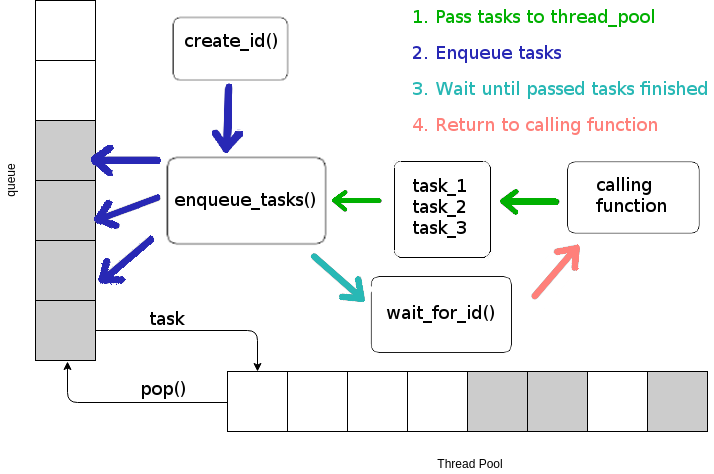
\includegraphics[width=0.5\textwidth]{img/pool_queue.png}
	\caption{Workflow of task enqueueing and execution in the thread pool}
	\label{fig1}
\end{figure}

\subsection{Waiting for Tasks}
As mentioned before, the thread pool provides the functionality to let the calling function participate in the task execution and wait until all passed tasks are processed. To wait for a set of tasks, it is not sufficient to look firstly in the priority queue for the tasks and then in the state of the thread pool, since popping tasks out of the queue is not an atomic operation. Consequently, tasks can have a state between being enqueued in the queue and being executed by a thread.

To solve this problem, we implement the waiting for a set of tasks using a slot-map. In Figure 3, we show the concept of our slot-map. During the enqueueing process of tasks, a set of tasks is mapped to a slot in the slot-map. Each slot contains a number of open tasks to be finished and a generation counter. We name the number of open task \emph{openTaskCount} and the generation counter \emph{genCount}. Every time a set of tasks is enqueued, a slot with $openTaskCount = 0$ is selected and the \emph{genCount} increases. Every time a thread finishes a task, the $openTaskCount$ of the referred slot is decreased. As mentioned before, multiple tasks can refer to a single handle. This handle also refers to a slot and has additionally assigned a generation value. The waiting algorithm loops over the following conditions before returning to the calling function: It checks if the number of open tasks is zero or if the generation counter of this slot has changed. If one of these conditions is true, the waiting algorithm returns to the calling function.

To clarify the procedure of the waiting algorithm, we consider the second slot in Figure 3. The tasks $10, 12, $ and $13$ as well has the first handle refer to this slot. Consequently, these tasks were enqueued referring to the first handle. Before any of the three tasks is processed, the slot has the following state: $openTaskCount = 3$ and $genCount =  2$. Since the waiting thread does not know when tasks are executed due to the asynchronous behaviour, the waiting algorithm starts looping as long as the following condition is true: $openTaskCount \neq 0$ \&\& $genCount = 2$. For each finished task, $openTaskCount$ is decreased. It is not sufficient to check only $openTaskCount \neq 0$, since the slot can be reused before the waiting algorithms noticed that $openTaskCount = 0$. Consequently, we check if the slot stays on the same generation. If the slot is reused, $genCount$ increases and the second part of the condition returns false.

Since $openTaskCount$ has to be altered from different threads the required decrements are ensured to be atomic. This is in opposition to the usual goal of slot-maps to improve cache locality. Atomics on x86 usually prevent their whole cache line from being used while they are changed. Thus a sparse distribution of slots should reduces collisions. To quantify this difference the baseline implementation searches for free slots linearly from the beginning, while an alternative approach tries to distribute the slots over multiple cache lines. In Figure \ref{fig10}, we show implementations for both search approaches.

\begin{figure}
	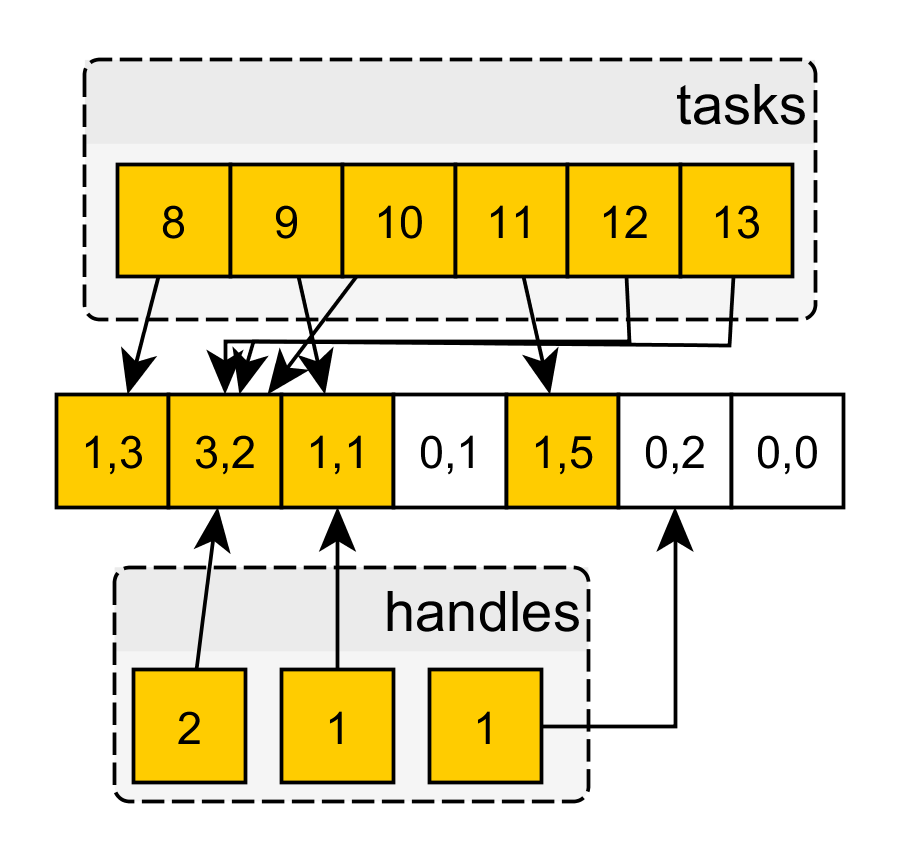
\includegraphics[width=0.4\textwidth]{img/waitingconcept.png}
	\caption{Concept of waiting for tasks using a slot-map}
	\label{fig2}
\end{figure}

\subsection{Managing Thread States}
As mentioned before, accessing the same memory location from different threads may lead to race conditions, which means the program behaviour depends on the accessing order of the threads. For example, while one thread updates data at a specific memory location, another thread writes into the data, which results to inconsistency. In Section 2, we presented two approaches to handle multithreaded access to the same memory location, mutex threads and atomic operations and we state where those approaches are used in our implementation. In this subsection, we focus on atomic operations to manage thread states. We consider the following steps for a thread to update its state. At first, the current state has to be checked and, depending on the current state, it has to be updated. If these steps are implemented using an if statement and an update function, the complete procedure is not atomic. Consequently, another thread can update the state between check of the current state and update. To avoid this, we use the function \emph{atomic\_compare\_exchange\_strong} \cite{atomicstrong} of the stdatomic library. This function combines the check and update in one atomic procedure. We implemented every thread state access with this function to ensure atomic thread state updates. 

\begin{figure}
	\begin{lstlisting}[style=CStyle]
	size_t ind = 0;
	// linear search, compact slot usage
	for(; ind < pool->task_state_capacity && pool->task_group_states[ind].task_count; ++ind);
	// distributed over different cache lines
	for(; pool->task_group_states[ind].task_count; ind = (ind + 8) % MAX_NUM_TASKS);
	\end{lstlisting}
	\caption{Different implementations for slot searching}
	\label{fig10}
\end{figure}

This approach enables efficient dynamic and lazy resizing of the thread pool. When the number of threads is reduced, the now redundant threads are marked to finish after completing their current task. If later on the number is increased again, still running but marked threads can be enabled again ensuring that few threads have to be created and that the number of running threads will not temporarily exceed the requested size. 
 After presenting the enqueueing, processing, and waiting for tasks, we show the second component of our thread pool system, the performance monitoring.

\subsection{Performance monitoring}
The performance monitoring component of the thread pool system is responsible for collecting data about threads, tasks, and the thread pool instance. We will use the information collected in this component for analysis and performance optimization in later stages. As mentioned before, the performance monitoring is an optional component, since evaluating the following statistics can reduce the execution performance of our thread pool. We divide the collected statistics into the sections \emph{task statistics}, \emph{thread statistics}, and \emph{thread pool statistics}.

\subsubsection{Task Statistics}
Collecting statistics about the time tasks spend in the priority queue or during the execution is useful to tune the thread pool configuration for better performance results. In Table \ref{tab2} we show the statistics that are collected for each task.

\begin{table}[htbp]
	\caption{Task statistics with their internal names and descriptions}
	\begin{center}
		\begin{tabular}{ l l }
			\hline
			\textbf{Statistic name}&\textbf{Description}\\
			\hline
			enqueue\_time & Time when the task was enqueued \\
			execution\_time & Time when the task execution begins \\
			complete\_time & Time when the task execution is finished \\
			\hline
		\end{tabular}
		\label{tab2}
	\end{center}
\end{table}

How long a task waits in the queue before being executed is a good metric to adjust task priority or the thread pool size. For example, if an enqueued task with priority 0 still has a large difference between \emph{enqueue\_time} and \emph{execution\_time}, the thread pool size may be too small. Otherwise, if a large number of tasks with low priority have small differences between \emph{enqueue\_time} and \emph{execution\_time}, this may indicate that the thread pool size is too large. A better indicator of not optimized thread pool sizes are statistics per thread.

\subsubsection{Thread Statistics}
As mentioned before, adjusting the thread pool size based on task statistics may not be very precise. Consequently, collecting statistics per thread is necessary for a good evaluation of the relation between tasks and threads. In Table \ref{tab3}, we show our statistics collected for each thread in a thread pool instance.

\begin{table}[htbp]
	\caption{Thread statistics with their internal names and descriptions}
	\begin{center}
		\begin{tabular}{ l l }
			\hline
			\textbf{Statistic name}&\textbf{Description}\\
			\hline
			waiting\_time & Time the thread spend waiting (ms) \\
			busy\_time & Time the thread spend executing tasks (ms)\\
			task\_count & Number of tasks the thread has executed \\
			\hline
		\end{tabular}
		\label{tab3}
	\end{center}
\end{table}

The \emph{busy\_time} of a thread strongly depends on the executed tasks and therefore is a metric that gives less information about the thread pool itself. In contrast, the \emph{waiting\_time} is a good indicator to reveal less used threads in the thread pool to determine an optimal amount of threads for the current use case. Furthermore, the \emph{task\_count} of thread compared to the number of tasks processed by the thread pool indicates the degree of usage of the thread. To give further possibilities for optimizing the thread pool, we collect statistics for each thread pool instance.

\subsubsection{Thread Pool Statistics}
To consider the thread pool instance, an important metric is the average waiting time of tasks. In order to optimize the thread pool size, a balanced relation between the waiting time of tasks and the number of threads must be found. Furthermore, at a specific time, the relation between enqueued and completed tasks can be interesting. In Table \ref{tab4}, we show our statistics collected for each thread pool instance. We will use these statistics to adapt our thread pool implementation to different use cases later on.

\begin{table}[htbp]
	\caption{Thread pool statistics with their internal names and descriptions}
	\begin{center}
		\begin{tabular}{ l l }
			\hline
			\textbf{Statistic name}&\textbf{Description}\\
			\hline
			working\_time & Time the thread pool runs (ms) \\
			task\_complete\_count & Number of tasks the thread pool has completed\\
			task\_enqueued\_count & Number of tasks the thread pool has enqueued \\
			avg\_complete\_time & Average time span from enqueueing until \\
			& execution of tasks \\
			avg\_wait\_time & Average time of tasks spend in the queue \\
			\hline
		\end{tabular}
		\label{tab4}
	\end{center}
\end{table}

\subsection{Testing and Memory Check}
As last aspect of our implementation, we show how we test the thread pool and how we ensure to avoid memory leaks. Since GeckoDB already uses GTest \cite{sen2010quick} for unit testing, we also wrote our test using this framework. GTest provides a simple, powerful library to perform unit tests in C++. We wrote unit tests for the priority queue, the thread pool itself and the performance monitoring. As mentioned before, we use functions from the stdatomic library of c. Using this library in GTest results in compiler errors with GCC, since the c atomic implementation differs from the c++ one of the standard library and the GCC developers will not fix this issue. Consequently, we wrote a workaround not using the c stdatomic library in the GTest compilation unit.

Since c as low level language does not have an own memory management, memory leaks may occur using heap space allocations. To find and remove all memory leaks in our implementation, we use the tool \emph{valgrind}, which offers different functionalities to find race and jump condition and to count unfreed heap blocks. We found memory leaks in our priority queue tests and also in the deallocation of thread pool instances. In the following sections, we show our experimental setup and the results of our evaluation.

\section{Experimental Environment}
In this section, we present our experimental environment focusing on the design of our benchmarks and the system configuration we used to evaluate our thread pool implementation.

\subsection{Evaluation Setup}
In our evaluation setup, we focus primarily on the comparison of our thread pool against the baseline implementation in BOLSTER, that creates new threads at runtime for each request. We simulate calls of BOLSTER primitives with different thread pool and task configurations and compare the results against the baseline.

Additionally, we evaluate the metrics for threads, tasks and the thread pool mentioned in Section 3.F regarding the thread pool and task configuration used in the BOLSTER primitives. To evaluate optimal configurations for the thread pool, we consider the relation between waiting and completion time of  thread pool instances with different sizes.

%Furthermore, we compare the scope and usage of our thread pool against an existing implementation \emph{Threading Building Blocks (Intel TBB)} \cite{kim2011multicore} written in C++. Since Intel TBB uses completely different approaches to parallel the execution of tasks, a direct performance comparison may not lead to reliable results. Therefore, we evaluate the usage and the scope both implementations give.

\subsection{Experimental Configuration}
%\textbf{TODO: Change!}\\The operating system is Ubuntu 17.04 with linux kernel
%version 4.13 running in a virtual machine on an Intel Core i7-6700HQ, 4x 2.6 GHz
%(Skylake) and 8GB DDR3 RAM running on 1600Mhz. We reduce the number of cores of
%the virtual machine to 4 instead of 8 virtual cores of the CPU. The CPU has
%256KB L1 cache, 1MB L2 cache, and 6MB L3 cache. All benchmarks have been
%repeated three times and a median value of all repetitions is being used for evaluation.

For testing purposes we used primarly Linux setups, for one Ubuntu 17.04
(linux 4.13) in an virtual machine environment, second Archlinux (linux
4.17.3-1) running native, both updated on stable branch. Tests have also been
conducted on Windows 10 and macOs HighSierra machines.

In our setups Sky- and Kabylake aswell as Ryzen processors have been used with memory
ranging from 8 to 24 GB of both DDR3-SODIMM and DDR4-SODIMM. 
All benchmarks have been repeated three times and a median value of all
repetitions is being used for evaluation.

\section{Evaluation}
In this Section, we present the results of our evaluation according to the setup we stated in the previous section. We start with an introduction of the benchmark methods to compare our thread pool against the baseline implementation and present the results. Furthermore, we show the relation of waiting time and completing regarding different thread pool configurations.

\subsection{Validity of Results} 
Before presenting our evaluation results, we
give some preliminaries about the validity of our results. At first, all
measurements are executed on all machines we listed in our experimental
configuration, but in this work we present only the results measured on
Archlinux with kernel 4.17.3-1 and 24 GB DDR4-SODIMM. We decided to use this
system, since it is running a current kernel version and not in a virtual
environment. Additionally, we use gnuplot to generate diagrams from our results,
consequently using a windows machine is not optimal.

Secondly, the measured results represent the usage of our thread pool implementation, but may differ strongly in other applications. Depending on the number of threads used outside the thread pools and the ability to parallelize work, the performance may increase less than shown in our tests.

Thirdly, measuring multi threading performance highly depends on the current workload of the system and the scheduler. We determine this in our evaluation since tests differ strongly in their results. Although we make average measurements for each benchmark, these represent the performance increase at the current system workload.

\subsection{Comparison against Baseline Implementation}
As most important aspect of our evaluation, we compare our thread pool against an approximated version of the baseline implementation. To justify the performance comparison results, we present the different benchmark implementations in detail before we show the evaluation results.

\subsubsection{Benchmark Implementation}
Since BOLSTER is deeply integrated into GeckoDB and the workload and usage of multi threading depends on the graph data in the system, we can not directly use the BOLSTER implementation for our evaluation. Thus, we extracted the respecting code parts into an own implementation and use this for a direct comparison against one that uses our thread pool. 

In Figure \ref{fig4}, we show the approximated version of the BOLSTER multi threading code that we use as baseline implementation. In our benchmark. the method \emph{cmp\_baseline} is called multiple times with a different \emph{numThreads} parameter. Within each call, \emph{numThreads} threads are created and all of these execute the benchmark method \emph{work\_large}, that calculates a huge amount of exponential values in a loop. After the calling thread takes part in execution, it waits until all created threads are joined. The elapsed processing time is measured from the begin of the method until the join of all threads finished.

\begin{figure}
	\begin{lstlisting}[style=CStyle]
		void cmp_baseline(int numThreads)
		{
			struct timespec begin, end;
			clock_gettime(CLOCK_MONOTONIC, &begin);
			
			double results[numThreads];
			
			pthread_t threads[numThreads];
			for (int tid = 1; tid < numThreads; tid++)
			{
				results[tid] = (double)(tid+1);
				pthread_create(&threads[tid] , NULL, 
					&work_large, &results[tid]);
			}
			
			// Let the calling thread process one 
			// task before waiting
			work_large(&results[0]);
			
			for (int tid = 1; tid < numThreads; tid++) {
				pthread_join(threads[tid], NULL);
			}
			
			clock_gettime(CLOCK_MONOTONIC, &end);
			test_results_baseline[numThreads] +=
				__get_time_diff(&begin, &end);
		}
	\end{lstlisting}
	\caption{Baseline multi threading implementation extracted from BOLSTER}
	\label{fig4}
\end{figure}

\begin{figure}
	\begin{lstlisting}[style=CStyle]
		void cmp_pool(int numThreads)
		{
			thread_pool_t* pool = 
			thread_pool_create(numThreads, 1);
			
			struct timespec begin, end;
			clock_gettime(CLOCK_MONOTONIC, &begin);
			double results[numThreads];
			thread_task_t tasks[numThreads];
			
			for(int i = 0; i < numThreads; ++i)
			{
				results[i] = (double)(i+1);
				tasks[i].args = &results[i];
				tasks[i].routine = work_large;
				thread_pool_enqueue_task(&tasks[i], pool, 
					NULL);
			}
			
			thread_pool_wait_for_all(pool);
			
			clock_gettime(CLOCK_MONOTONIC, &end);
			test_results_pool[numThreads] += 
				__get_time_diff(&begin, &end);
			
			thread_pool_free(pool);
		}
	\end{lstlisting}
	\caption{Thread pool benchmark to compare against baseline implementation}
	\label{fig5}
\end{figure}

To compare against the presented baseline implementation, we developed a method that does the same amount of calls of \emph{work\_large} as the baseline, but uses a thread pool instance instead of creating new threads. In Figure \ref{fig5}, we show this implementation called \emph{cmp\_pool} that creates and fills tasks and enqueues these into a thread pool instance. Since we assume, that the thread pools are reused for multiple requests, we exclude the thread pool creation and deallocation from the time measure. Consequently, only creating and processing tasks is included in the considered elapsed time. 


\subsubsection{Evaluation Results}
In our performance comparison, both implementations are executed three times with $4, 8, 16, 32$ as \emph{numThreads} parameter and the summed results are divided by three. We consider a number between $4$ and $32$ as a useful amount of threads to reach a sufficient performance increase due to parallelization, but also to have the possibility to debug and profile them. 

In Figure \ref{fig6}, we show the comparison results of both mentioned implementations and the different \emph{numThreads} parameters. Our thread pool implementation is faster than the baseline for all \emph{numThreads} parameters. Based on Figure \ref{fig6}, we make the following conclusions.  
Firstly, compared to strict processing workload, create, and later on join threads, consumes much time. Our thread pool implementation reaches up to a multiple of performance increase compared to the baseline. Since the creation and join of threads is the main difference between both tests, reusing threads will lead to this noticeable performance increase. 

Secondly, the task creation and enqueuing have only slight impact on the performance, since the baseline does not include these operations, but is still clearly slower than the thread pool implementation. 

\begin{figure}
	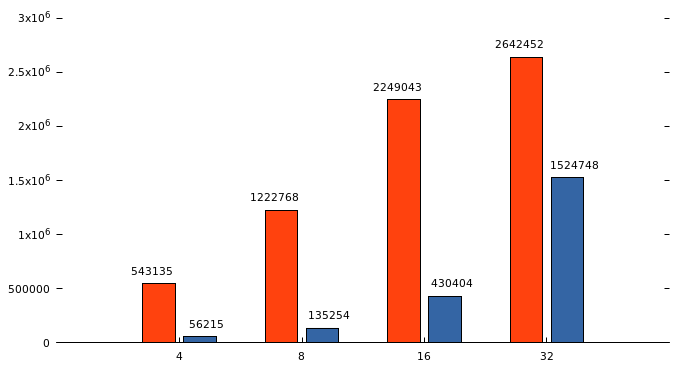
\includegraphics[width=0.5\textwidth]{img/pool_baseline.png}
	\caption{Time measures in nanoseconds of thread pool (blue) and baseline (orange) implementation with different numbers of threads.  }
	\label{fig6}
\end{figure}

\subsection{Waiting Time Evaluation}
As mentioned before, instead of implementing explicit scheduling to assign tasks to threads, we use the \emph{first come first serve} approach. Each thread that currently has no task, checks the priority queue to pop a new task in a loop. Since our priority queue manages the memory access from different threads using a mutex thread, the queue is locked while a thread asks for a task. Consequently, in large thread pools, the accessing time of the priority queue may increase along with the waiting time of threads. To examine this behaviour with increasing thread pool size, we measure the average waiting time of thread pools with different sizes.

To further test the performance of the task-completion system, in particular the previously mentioned wait-slot acquisition, the main thread periodicity has to wait for a specific task to finish and the total utilization is measured.

\subsubsection{Benchmark Implementation}
To examine the waiting time behaviour of larger thread pools, we use a similar implementation than the \emph{cmp\_pool} method, which creates 10000 tasks at different thread pool sizes. Again, we consider sizes from $4$ to $32$ threads as useful test case and take the average value of three measurements. To measure waiting and completion time, we use the monitoring component of our system and evaluate the thread pool statistics of each instance. 

\subsubsection{Evaluation Results}
In Figure \ref{fig7}, we show the relation of waiting and completion time of different thread pool sizes. The waiting time is, compared to the completion time, very small and nearly constant for all considered thread pool sizes. From this observation, we draw the following conclusions for our \emph{first come first serve} scheduling approach. Firstly, constant average waiting time indicates only small performance decreases due to priority queue locking. Secondly, even for $32$ threads in one pool instance, the waiting time occupies only a small fraction of the completion time, which indicates good thread usage.  Thirdly, the execution performance increases along with the thread pool size, which shows that even for $32$ threads, parallelization leads to faster task execution. 

\begin{figure}
	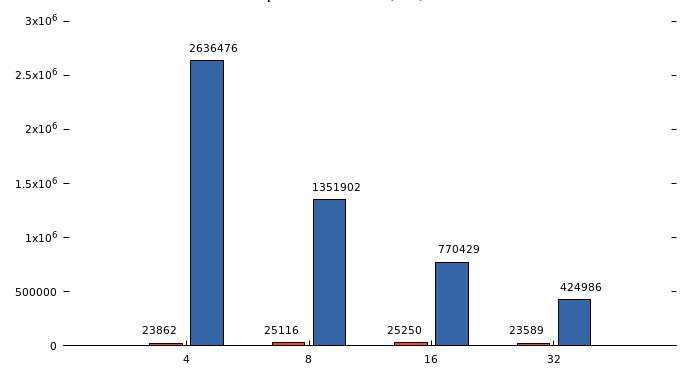
\includegraphics[width=0.5\textwidth]{img/pool_avg.png}
	\caption{Relation between waiting time (orange) and completion time (blue) of thread pools with different sizes processing 10000 tasks}
	\label{fig7}
\end{figure}

As mentioned before in this section, the performance results depend on the current workload of the system, as seen by the waiting time shown in Figure \ref{fig7}. Although the priority queue locking by the mutex thread should increase the waiting time slightly with bigger thread pool sizes, the last measuring point is lower than the previous points. 

The selection strategy of wait-slots has only a small impact on occupation, as seen in Figure \ref{fig8}. The uniform distributions advantage amounts to $0.1\%$ across different numbers of threads and is far overshadowed by differences in the threads to tasks ratio.

In Figure \ref{fig9}, we show that the lock-free priority queue performs better. With a difference in utilization of $2\%$ when using only two threads the improvement over our mutex based implementation is not insignificant. A total occupation of over $99.5\%$ also demonstrates that most overhead in our implementation comes from the priority queue when supplying a balanced stream of tasks. With an increase in available threads the performance of the mutex solution further decreases, while the lock-free queue-variants utilization remains nearly constant.


\begin{figure}
	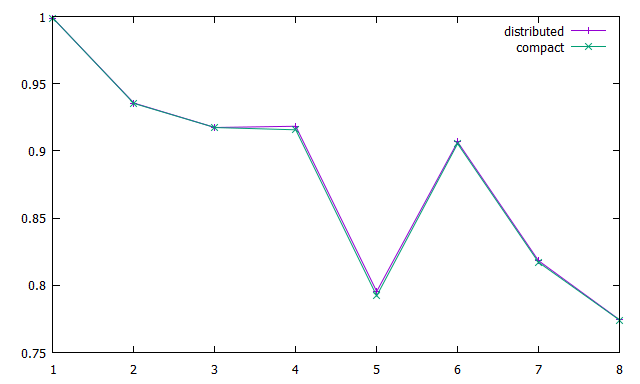
\includegraphics[width=0.5\textwidth]{img/slot_distr.png}
	\caption{Utilization \% with different slot distribution strategies}
	\label{fig8}
\end{figure}

\begin{figure}
	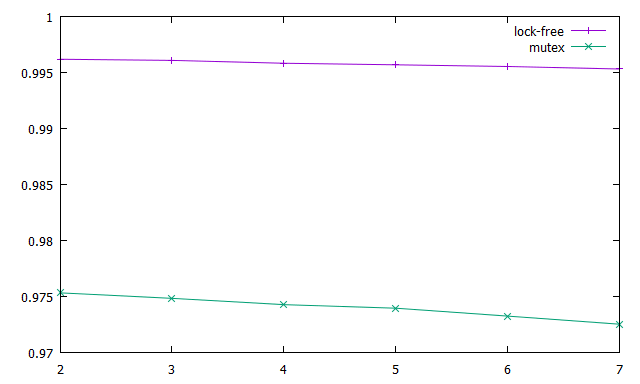
\includegraphics[width=0.5\textwidth]{img/lock_free.png}
	\caption{Comparison of Utilization \% of the lock-free queue versus mutex based heap}
	\label{fig9}
\end{figure}

\subsection{Summary}
As last step of the evaluation, we summarize our results and compare them to the requirements of GeckoDB. As mentioned before, our implementation reaches better performance than the baseline regarding our specific tests. Consequently, we solved the task for implementing and integrating the thread pool into BOLSTER to reach at least the baseline performance. Additionally, using our thread pool implementation solves the problem, that debugging and profiling with a huge number of threads is not possible. 

Although a small and constant waiting time was not a requirement for integration into GeckoDB, we ensure that assigning many tasks works fast for different thread pool sizes. Regarding the performance and also the design requirements of GeckoDB and BOLSTER, we fulfil these requirements and successfully implemented and evaluated our thread pool implementation.

The choice of a different priority queue data structure presents an opportunity for further optimizations, in particular to scale well with large amounts of threads.

\section{Related Work}
Implementing multi threading can be realised using different approaches from spawning new threads to reuse them in thread pools. Pyarali et al. show that a thread pool model can significantly improve system performance and reduce response time \cite{pyarali2001evaluating}. They present different approaches to implement thread pools and show the dependency on use cases of these implementations.

Schmidt et al. present different implementations of multi threading, including two types of thread pools. They distinguish between the \emph{Worker Thread Pool Architecture} and the \emph{Leader/Follower Thread Pool Architecture} \cite{schmidt1998evaluating}. In the first approach, an IO-thread selects a connection, reads the requests and dispatches the tasks to an array of threads. Drawbacks of this system are excessive context switching effort along with synchronization required to manage the request queue. In the second approach, one thread of the pool becomes the leader and does the reading of the task into an internal buffer. If the request is valid, the thread itself processes the task and a follower thread becomes the new leader. This approach minimizes the context switching effort compared to the first one.

Along with the design of thread pool systems, the performance strongly depends on the number of threads used in a thread pool. Xu et al. present a performance study for a set of performance metrics combined with a heuristic algorithm for dynamic resizing of thread pools \cite{xu2004performance}. They show the correlation between average task idle time and the throughput of thread pools and present the effectiveness of dynamically adjusting the number of threads.

Compared to heuristically adjust the number of threads, Ling et al. formalized the problem of finding the optimal number of threads by establishing mathematical relationship among optimal thread pool size, system load and the associated costs \cite{ling2000analysis}. They show the applicability of their model and plan to further examine it based on additional metrics.

\section{Conclusion and Future Work}
In this work, we describe our implementation of a thread pool system. We present in detail the implementation and show our evaluation results containing a comparison against the baseline implementation and the waiting time behaviour over different thread pool sizes. Within our implementation, we state the differences of parallel memory access as well as the problem of implementing synchronous waiting for a set of tasks.

As presented in the evaluation, our thread pool implementation reaches better execution performance than the baseline because of avoiding the creation of short living threads for each request. We measured the average time threads spent waiting in different thread pool sizes and present, that even for a size of $32$ threads, the waiting time stays constantly small. Consequently, we conclude that using \emph{first come first serve} as scheduling approach leads to small waiting times and high execution performance. 

To sum up, our thread pool implementation fulfils all performance and design requirements of GeckoDB and BOLSTER and reaches even faster execution time than the existing implementation. In the future, we plan to make the following adaptations to our thread pool system. Firstly, we want to reduce the number of dynamic allocation, since heap allocations mostly are slower than stack allocations. Secondly, we want to examine the usage of existing priority queue implementations for our thread pool system. Thirdly, we plan to integrate a dynamic resizing function based on the collected statistics of the performance monitoring component. 

\bibliographystyle{splncs}
\bibliography{paper_thread_pool}

\end{document}
